\section{Имитационное моделирование}
В данной работе, для анализа полученных решений систем массового обслуживания с повторными вызовами и вызываемыми заявками используется имитационное моделирования. Построив имитационную модель системы, мы получаем возможность сравнить результаты ее работы с решением, что позволить оценить применимость полученных результатов, а так же облегчит получение численных характеристик, таких как коэффициент корреляции.
Моделирование систем массового обслуживания сводится к генерированию случайных времен с соответствующим распределением вероятности, по прошествии которого в модели наступит некоторое событие - приход заявки, окончание обслуживания и т.д.%, что называется дискретно-событийным подходом.

Реализованная имитационная модель, как программный продукт, разрабатывалась с возможностью расширения ее функционала для предоставления возможности тонко настраивать параметры моделирования и без препятствий извлекать полученные результаты в виде распределения вероятности для последующего анализа. В этих целях, программа реализована при помощи объектно ориентированного подхода, так как данный подход позволил выстроить работу программы на уровне абстракций, что и дает возможность легкого расширения функционала и реализации моделирования других систем массового обслуживания.

\subsection {Объектная модель предметной области}
Для того, чтобы построить объектную модель предметной области программы, рассмотрим  объекты систем массового обслуживания, используемые в данной работе:
\begin{itemize}
\item Заявка - объект, который поступает в систему, перемещается по ней и , в конечном итоге, покидает систему в течение моделирования.
\item Обслуживающий прибор - объект, принимающий на вход заявки и обслуживающий их. По окончании обслуживания заявки покидают прибор.
\item Орбита - скопление заявок, ожидающих повторного обращения на обслуживающий прибор.
\item Входящий поток - объект, генерирующий заявки, которые поступают в систему.
	\end{itemize}
 Поскольку, процесс работы модели заключается в перемещении заявок по системе, то в каждый момент времени моделирования $T_{mod}$ местонахождение каждой заявки и ее свойства могут меняться. В таком случае, необходимо отслуживать время, оставшееся до изменения состояния каждой заявки - $T_{del}$. В момент времени, когда $T_{del}$ достигает нуля,  происходит смена состояния заявки, и  $T_{del}$ обновляется объектом системы массового обслуживания, в которой она на данный момент находится. Среди событий , при которых происходит обновление задержки до обновления состояния заявки, выделим следующие:
\begin{itemize}
	\item Заявка покидает входящий поток - в данном случае в источнике генерируется новая заявка с задержкой, по истечении которой, она также покинет входящий поток.
	\item Заявка успешно поступила на прибор и начала обслуживаться - в этом случае обслуживающий прибор определяет заявки задержку, по истечении которой ее обслуживание закончится.
	\item При попытке поступить на прибор заявка застала его занятым обслуживанием другой заявки и отправилась на орбиту. По прибытии на орбиту, новая задержка заявки определяется как время, по истечении которого заявка покинет орбиту.
\end{itemize}
Исходя из вышеописанного, центральным объектом в предметной области является заявка.
\begin{figure}[H]
	\centering
	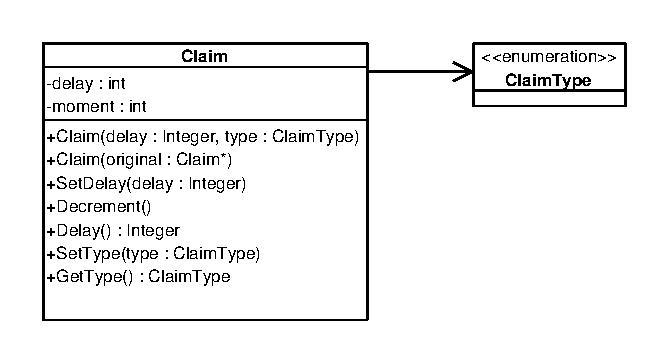
\includegraphics[scale=1]{claim_uml.eps}
	\caption{Класс Claim}
	\label{claim_uml}
\end{figure}
[Пояснение к Claim]

Для реализации подхода, базирующимся на постоянном обновлении состоянии заявок, находящихся в модели, предметная область базируется на общем интерфейсе, который реализуют все конкретные элементы рассматриваемых систем массового обслуживания. Его цель заключается в формализации изменения элемента  с каждым дискретным моментом времени в течение моделирования. Поскольку, сам объект системы массового обслуживания реализует данный интерфейс, то возможно использовать ее как входящий поток для другой системы.
\begin{figure}[H]
	\centering
	\includegraphics[scale=1]{processable_uml.eps}
	\caption{Общий интерфейс Processable для всех элементов системы массового обслуживания}
	\label{processable_uml}
\end{figure}
[Пояснение к Processable]

Для обеспечения среды, которой будет происходит моделирование, а именно - вестись подсчет прошедшего времени, вызов взаимодействие с реализацией интерфейса Processable и сбор статистики, введен глобальный объект Environment
\begin{figure}[H]
	\centering
	\includegraphics[scale=1]{environment_uml.eps}
	\caption{Глобальный объект Environment}
	\label{environment_uml}
\end{figure}
[Пояснение к Environment]

\subsection{Процесс моделирования}